% Adicione no preambulo do documento principal, caso ainda nao esteja carregado:
% \usepackage{graphicx}
% As pastas abaixo correspondem ao capitulo resultados.tex entregue anteriormente.

\begin{figure}[htbp]
    \centering
    \caption{Retorno por cardinalidade com controle dos ativos elegíveis.}
    \label{fig:resultados_ativos_comuns_gate3}
    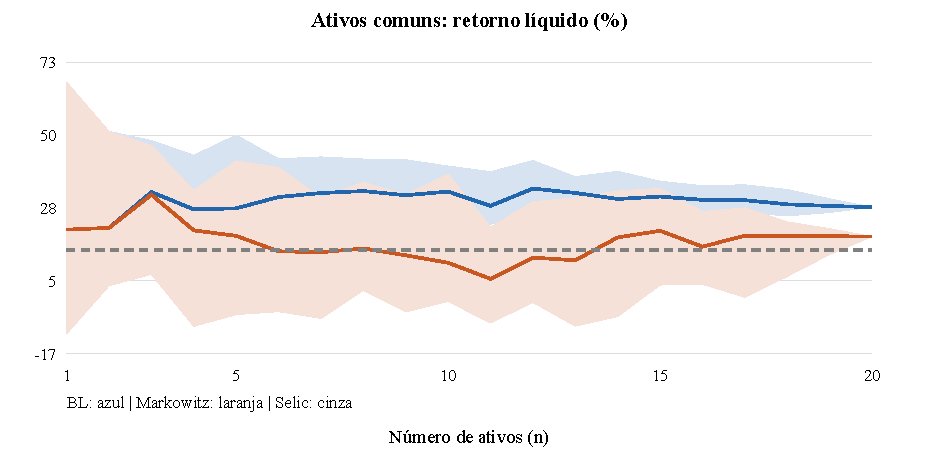
\includegraphics[width=\textwidth]{05_Resultados/figuras/ativos_comuns.pdf}
    \par\smallskip
    {\footnotesize Fonte: elaboração própria. Gate de três notícias. Faixas: percentis P10--P90 entre subconjuntos; não representam intervalos de confiança.}
\end{figure}

\begin{figure}[htbp]
    \centering
    \caption{Capital realizado em duas cardinalidades ilustrativas.}
    \label{fig:resultados_capital_gate3}
    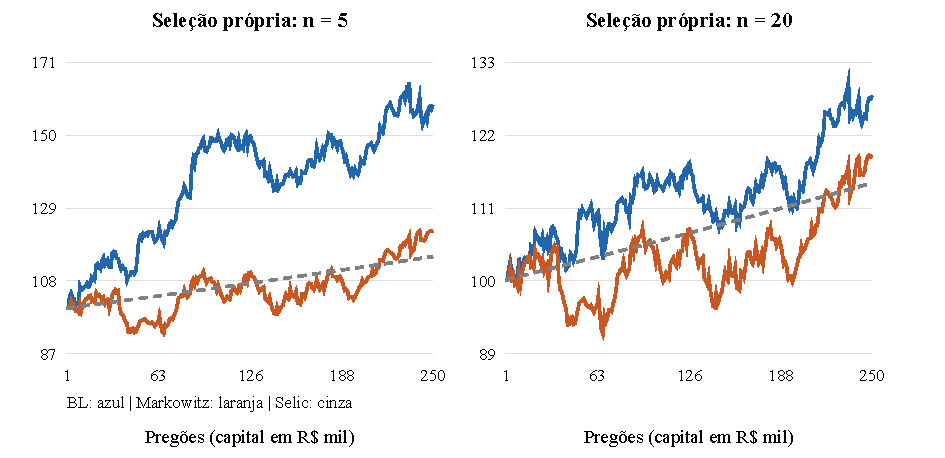
\includegraphics[width=\textwidth]{05_Resultados/figuras/trajetorias_capital.pdf}
    \par\smallskip
    {\footnotesize Fonte: elaboração própria. Gate de três notícias, capital inicial de R\$ 100 mil, rebalanceamento mensal e custos de 10 pontos-base. O caso $n=5$ é ilustrativo.}
\end{figure}
